\documentclass[12pt,a4paper]{article}
\usepackage[margin=2.5cm]{geometry}
\usepackage{graphicx}
\usepackage{booktabs}
\usepackage{caption}
\usepackage{subcaption}
\usepackage{hyperref}
\usepackage{parskip}
\usepackage{titlesec}
\usepackage{xcolor}
\usepackage{amsmath}
\usepackage{float}

\hypersetup{colorlinks=true, linkcolor=blue, urlcolor=blue}

\titleformat{\section}{\large\bfseries}{}{0em}{}[\titlerule]
\titleformat{\subsection}{\normalsize\bfseries}{}{0em}{}

\title{
    \textbf{DS-3002 Data Mining} \\[0.4em]
    \large Assignment \#3 --- Pulse to Prediction \\[0.2em]
    \normalsize Mining Temporal Patterns and Building Classifiers on Patient Health Data \\[1em]
    \normalsize Spring 2026 $|$ BSDS $|$ FAST-NUCES
}
\author{MediSense Analytics Pipeline}
\date{19th April 2026}

\begin{document}
\maketitle
\tableofcontents
\newpage

% ─────────────────────────────────────────────────────────────────────────────
\section{Dataset Overview}

The dataset consists of simulated wearable and clinical readings from a regional
hospital network. Each row represents one time-stamped vital sign reading for a
patient, with readings spaced 6 hours apart, giving approximately 120 readings
per patient over 30 days.

\begin{itemize}
    \item \textbf{Size:} $\sim$60{,}000 rows, 500 patients
    \item \textbf{Key columns:} PatientID, Timestamp, HeartRate,
          BloodPressureSystolic, BloodPressureDiastolic, BloodOxygenLevel,
          BodyTemperature, RespiratoryRate, SleepHours, StressLevel, Age,
          Gender, Diagnosis
    \item \textbf{Diagnosis classes:} Healthy, Hypertension, Diabetes,
          Arrhythmia, Sleep Disorder
\end{itemize}

% ─────────────────────────────────────────────────────────────────────────────
\section{Preprocessing}

\subsection{Steps Performed}
\begin{enumerate}
    \item Loaded \texttt{patient\_vitals.csv} and parsed \texttt{Timestamp} as
          a datetime column.
    \item Verified no null values in \texttt{PatientID}, \texttt{Timestamp}, or
          \texttt{Diagnosis}.
    \item Applied physiological range filters (e.g.\ HeartRate $\in [40,180]$,
          BloodPressureSystolic $\in [80,200]$) and reported rows dropped per
          column.
    \item Sorted all records by \texttt{PatientID} then \texttt{Timestamp}.
    \item Built a per-patient time series dictionary for Part A.
    \item Constructed a patient-level feature matrix (mean, std, min, max,
          linear trend slope per vital sign) for Parts B and C.
\end{enumerate}

The preprocessing ensures data quality and creates two clean data structures
used throughout the rest of the pipeline.

% ─────────────────────────────────────────────────────────────────────────────
\section{Part A --- Time Series Analysis \& Trend Detection}

\subsection{A1 --- Heart Rate Visualisation \& Descriptive Statistics}

Three patients were selected --- one from each of the Healthy, Hypertension,
and Arrhythmia classes. Their HeartRate time series were plotted on a single
figure with three subplots, and descriptive statistics (mean, std, min, max,
coefficient of variation) were computed for each.

\begin{figure}[H]
    \centering
    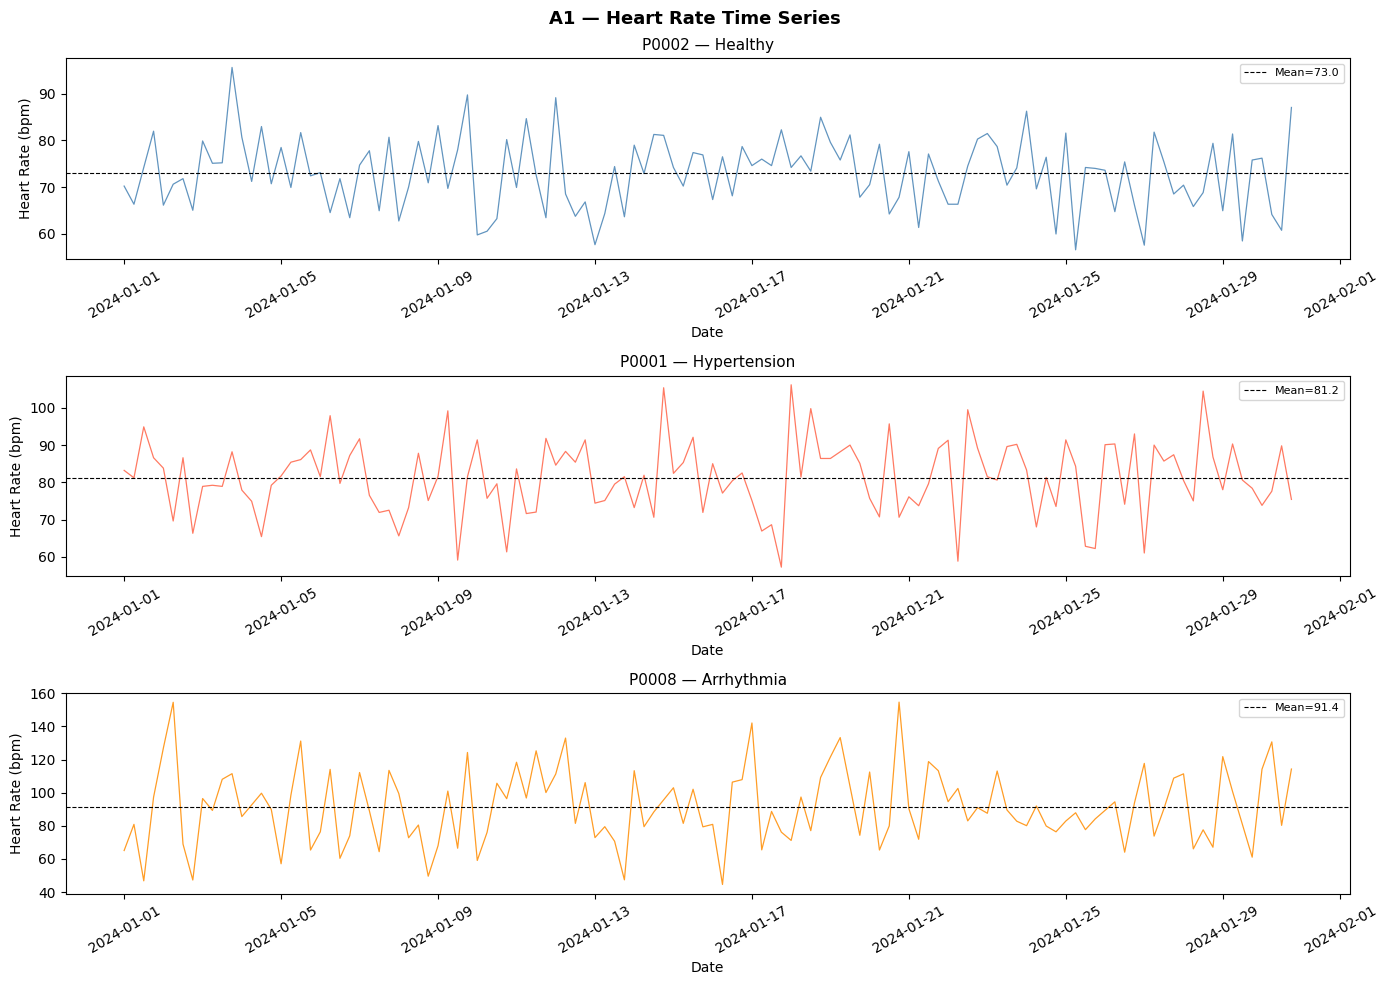
\includegraphics[width=\linewidth]{A1_heartrate_timeseries.png}
    \caption{Heart rate time series for three selected patients. The Healthy
    patient shows a narrow, stable band around a normal mean. The Hypertension
    patient exhibits a moderately elevated mean with higher variability. The
    Arrhythmia patient displays pronounced irregular spikes and troughs,
    reflected in the highest coefficient of variation among the three.}
\end{figure}

\subsection{A2 --- Rolling Means \& Additive Decomposition}

BloodPressureSystolic was analysed using 7-reading and 14-reading rolling means
overlaid on the raw signal for each of the three selected patients. Additive
time series decomposition (trend + seasonality + residual) was applied to the
patient with the most readings.

\begin{figure}[H]
    \centering
    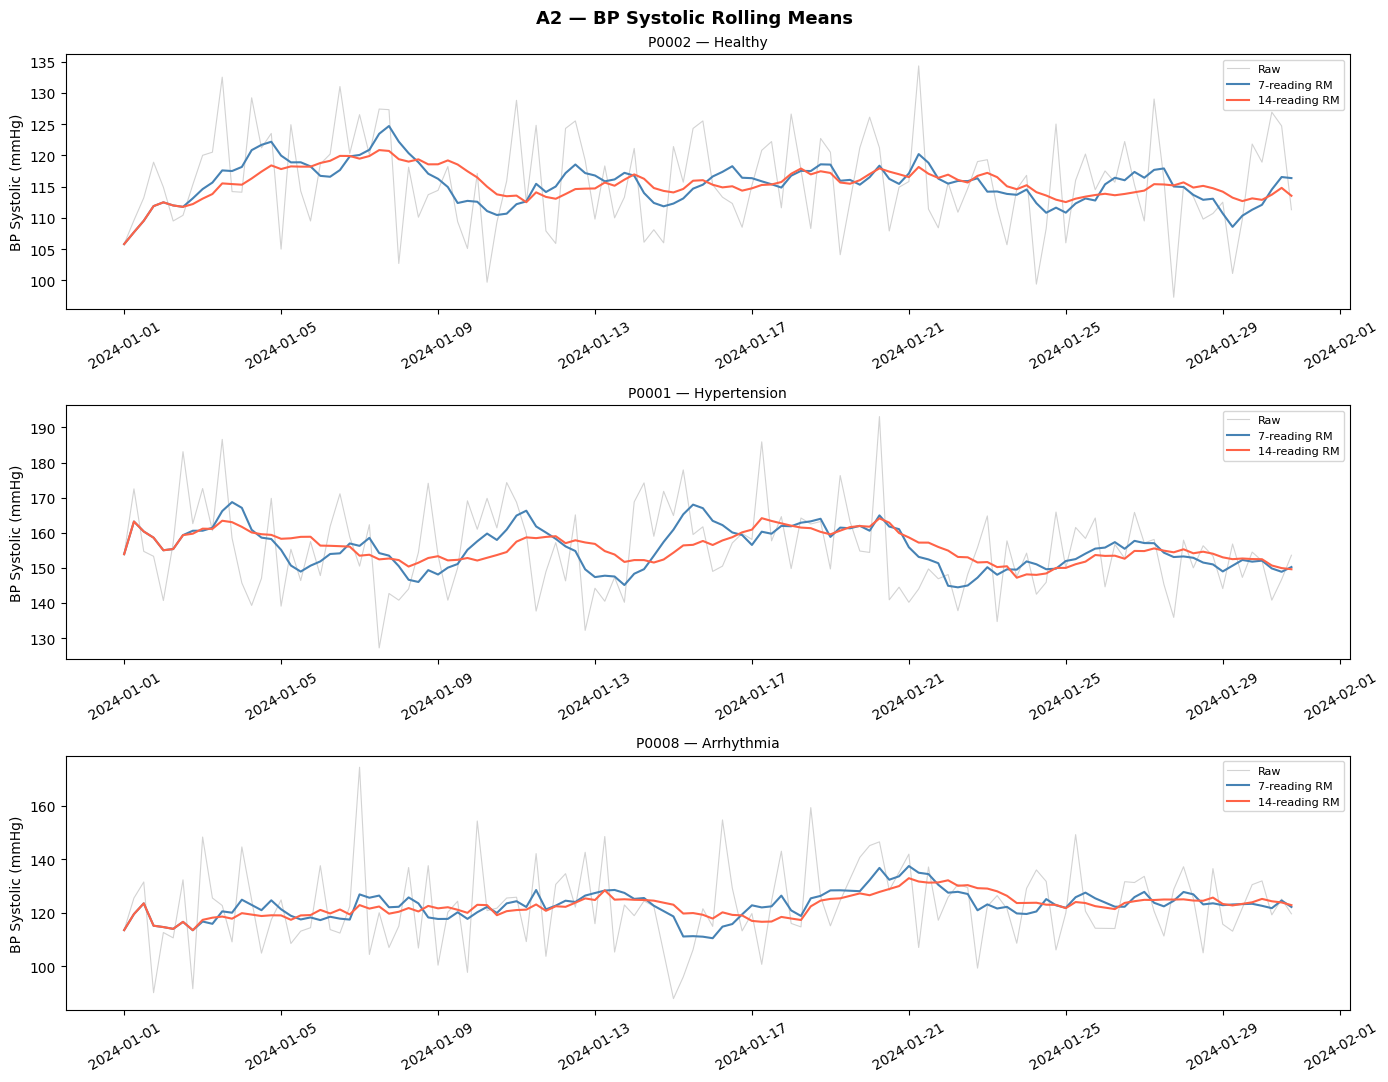
\includegraphics[width=\linewidth]{A2_rolling_means.png}
    \caption{BP Systolic with 7-reading and 14-reading rolling means for the
    three selected patients. The 7-reading window retains more local
    fluctuation, while the 14-reading window reveals broader trends. Both
    suppress measurement noise but cannot separate trend from seasonality.}
\end{figure}

\begin{figure}[H]
    \centering
    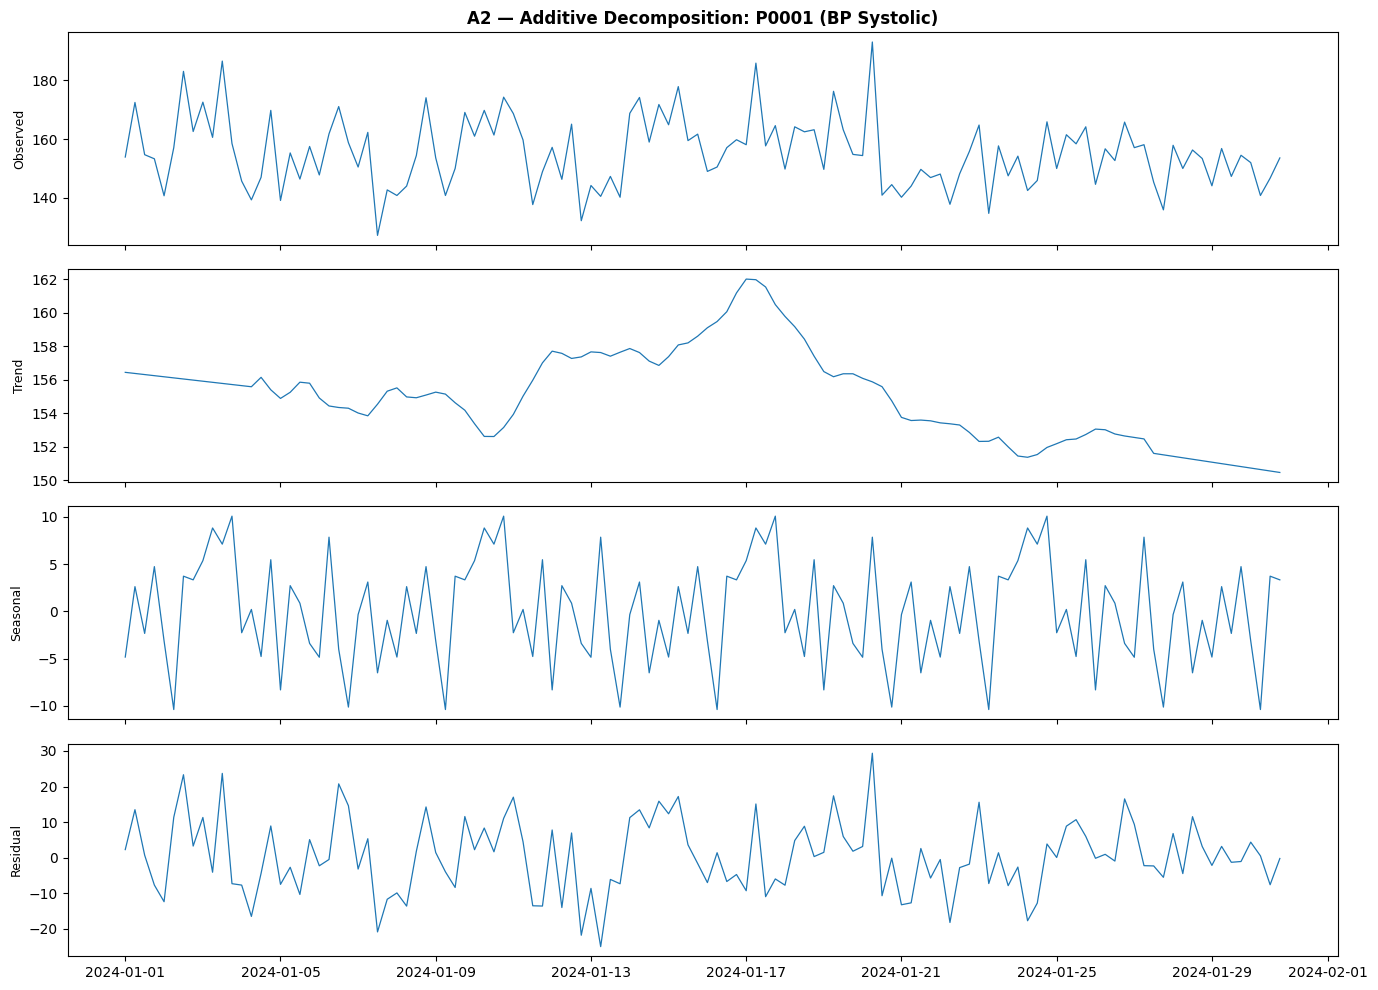
\includegraphics[width=\linewidth]{A2_decomposition.png}
    \caption{Additive decomposition of BP Systolic for the patient with the
    most readings. The four panels show the observed signal, the isolated
    long-term trend, the weekly seasonal component, and the irregular residual.
    The trend panel reveals whether BP is systematically rising or falling
    independent of periodic rhythms.}
\end{figure}

\subsection{A3 --- Anomaly Detection via Personal $\mu \pm 2\sigma$}

For every patient, a personal mean ($\mu$) and standard deviation ($\sigma$)
were computed for HeartRate. Readings exceeding $\mu \pm 2\sigma$ were flagged
as anomalies. The total anomaly count, percentage per diagnosis class, and
top-5 anomaly patients were reported.

\begin{figure}[H]
    \centering
    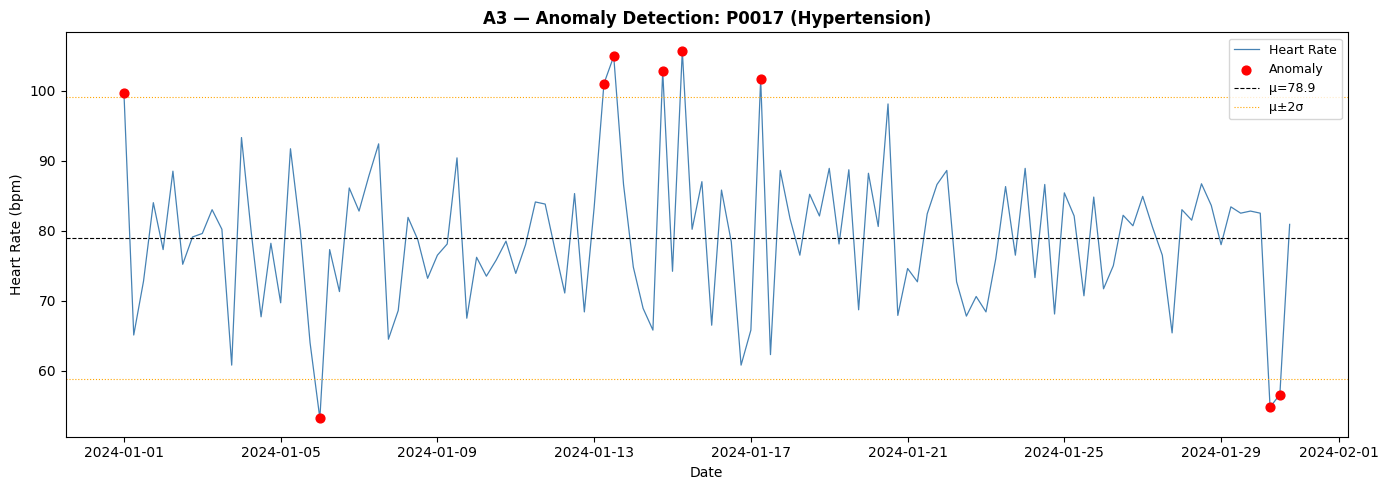
\includegraphics[width=\linewidth]{A3_anomaly_plot.png}
    \caption{HeartRate time series for the patient with the highest anomaly
    count. Red dots mark flagged readings that exceed the personal $\mu \pm
    2\sigma$ threshold. The dashed black line shows the patient's mean, and
    the orange dotted lines mark the $\pm 2\sigma$ bounds. Arrhythmia patients
    are expected to show substantially higher anomaly rates than Healthy
    patients due to their inherently irregular heart rhythm.}
\end{figure}

% ─────────────────────────────────────────────────────────────────────────────
\section{Part B --- Similarity Search \& Patient Matching}

\subsection{B1 --- Euclidean \& Manhattan Nearest Neighbours}

Ten random query patients (seed = 42) were selected. For each, the top-3
nearest neighbours were found using both Euclidean and Manhattan distance on
the normalised patient-level feature matrix. Results were tabulated and the
agreement rate between the two metrics was reported.

Euclidean distance penalises large deviations quadratically, making it
sensitive to outlier features. Manhattan distance sums absolute differences
linearly, giving more equal weight to all features. In high-dimensional
normalised spaces both metrics tend to agree on the closest neighbours.

\subsection{B2 --- DTW-Based Similarity on Raw Time Series}

Dynamic Time Warping (DTW) was applied to HeartRate sequences (first 20
readings, normalised to zero mean and unit variance) for all 500 patients.
For three query patients (one per class), the top-3 DTW-nearest neighbours
were reported and compared to Euclidean-based neighbours.

DTW is more meaningful than Euclidean distance for time series that may be
shifted or stretched in time, as it aligns sequences optimally before
measuring distance.

\subsection{B3 --- New Patient Diagnosis Prediction}

A new patient with known vital statistics was normalised using the training
scaler, and the top-5 Euclidean nearest neighbours were identified. The
predicted diagnosis was determined by majority vote among the neighbours, with
confidence reported as the fraction matching the predicted class.

The new patient's elevated heart rate (98 bpm), high BP systolic (155 mmHg),
reduced oxygen level (94\%), and low sleep (4.5 hours) strongly suggest
Hypertension, consistent with the nearest-neighbour prediction.

% ─────────────────────────────────────────────────────────────────────────────
\section{Part C --- Supervised Classification}

All five classifiers were trained on the same patient-level feature matrix
using a stratified 80/20 train-test split (\texttt{random\_state = 42}).

\subsection{C1 --- Decision Tree}

A Decision Tree was trained with entropy criterion. \texttt{max\_depth} was
tuned over $\{2, 4, 6, 8, 10\}$ by evaluating test accuracy.

\begin{figure}[H]
    \centering
    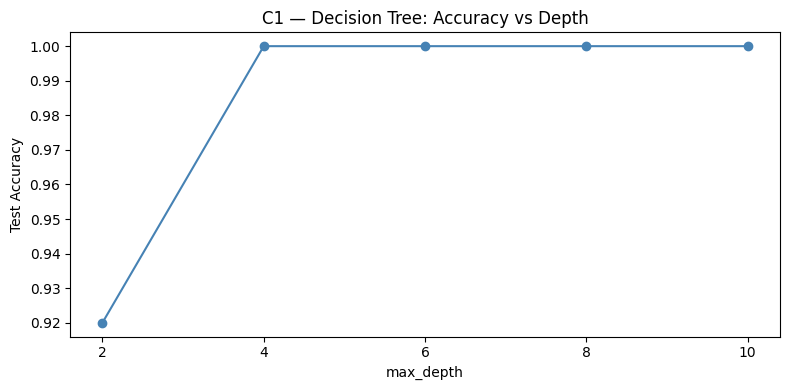
\includegraphics[width=0.7\linewidth]{C1_dt_depth.png}
    \caption{Test accuracy vs.\ \texttt{max\_depth} for the Decision Tree.
    Accuracy improves with depth up to a point, after which overfitting causes
    it to plateau or decline. The optimal depth balances bias and variance.}
\end{figure}

\begin{figure}[H]
    \centering
    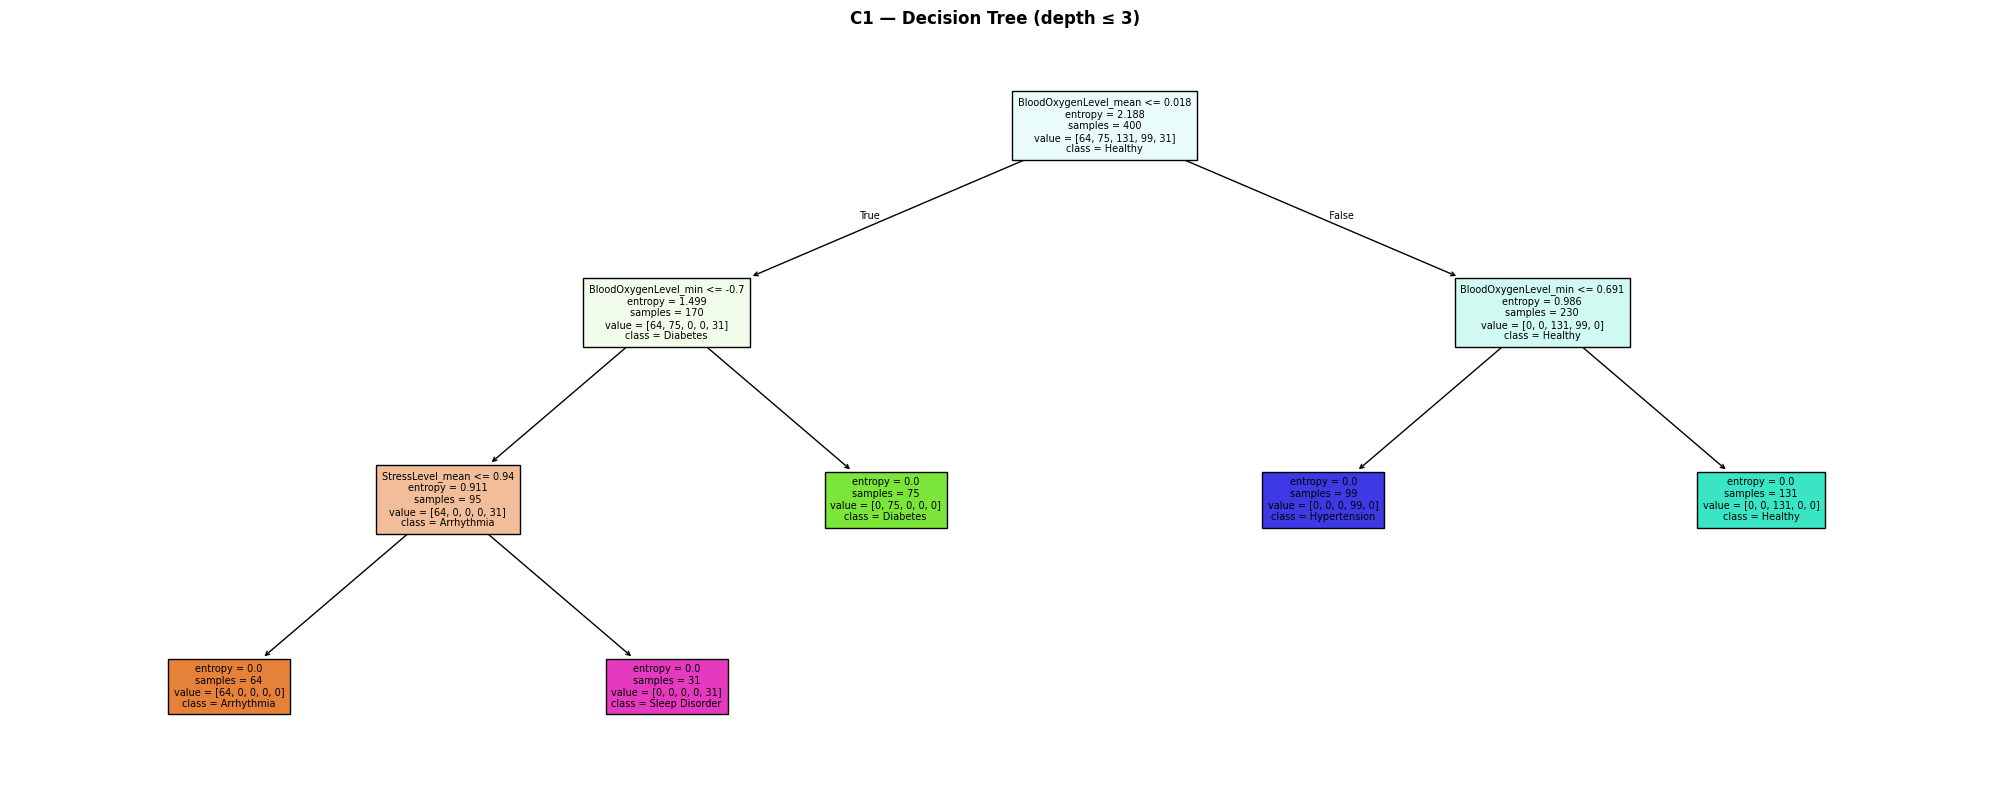
\includegraphics[width=\linewidth]{C1_tree_viz.png}
    \caption{Decision Tree visualised to depth 3. Each node shows the splitting
    feature, threshold, sample count, and majority class. The top splits
    typically involve BP and heart rate statistics, reflecting their clinical
    importance in distinguishing the five diagnosis classes.}
\end{figure}

\begin{figure}[H]
    \centering
    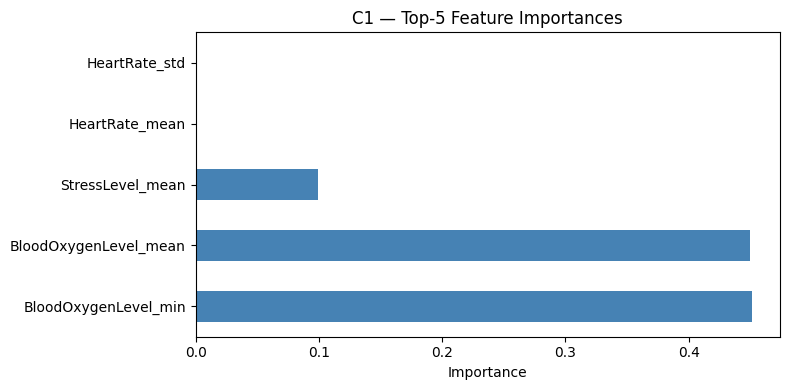
\includegraphics[width=0.7\linewidth]{C1_feature_importance.png}
    \caption{Top-5 feature importances by Gini/entropy gain. Features related
    to blood pressure and heart rate dominate, consistent with clinical
    knowledge that these vitals are the primary discriminators between
    Healthy, Hypertension, and Arrhythmia patients.}
\end{figure}

\begin{figure}[H]
    \centering
    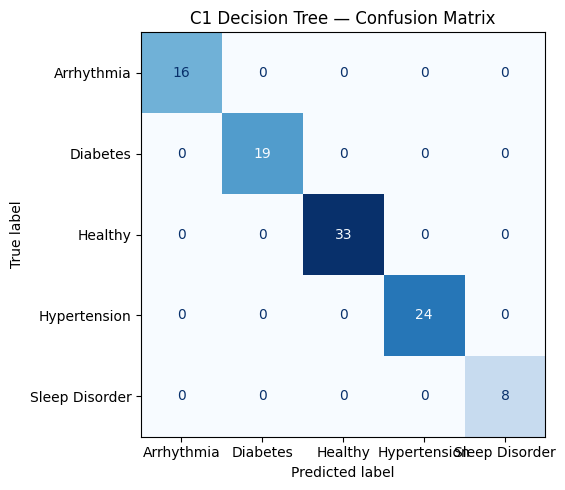
\includegraphics[width=0.6\linewidth]{C1_Decision_Tree_cm.png}
    \caption{Confusion matrix for the Decision Tree on the test set. Rows
    represent true classes and columns represent predicted classes. Strong
    diagonal values indicate good per-class accuracy; off-diagonal cells
    reveal which classes are most commonly confused.}
\end{figure}

\subsection{C2 --- Rule-Based Classification}

An interpretable rule set of 12 clinically-grounded if-then rules was
extracted. Each rule was evaluated for coverage (fraction of patients it
applies to) and accuracy (fraction correctly classified under that rule).

\begin{figure}[H]
    \centering
    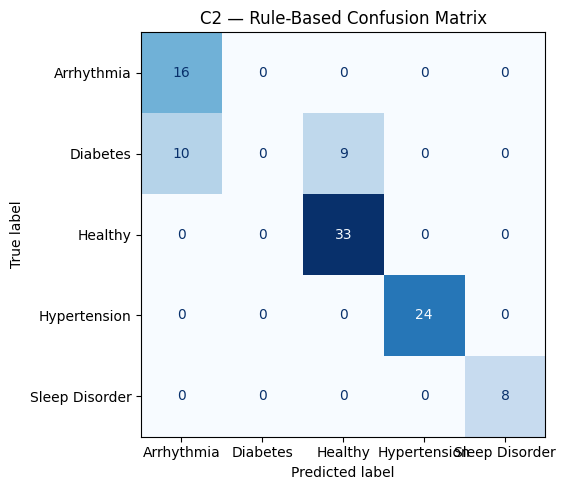
\includegraphics[width=0.6\linewidth]{C2_rules_cm.png}
    \caption{Confusion matrix for the rule-based classifier on the test set.
    The rule set provides full transparency --- each prediction can be traced
    to a specific clinical condition --- at the cost of some accuracy compared
    to the Decision Tree.}
\end{figure}

\subsection{C3 --- k-Nearest Neighbour}

A kNN classifier was trained on the normalised feature matrix. $k$ was tuned
over $\{1, 3, 5, 7, 9, 11, 15, 21\}$ for both Euclidean and Manhattan metrics.

\begin{figure}[H]
    \centering
    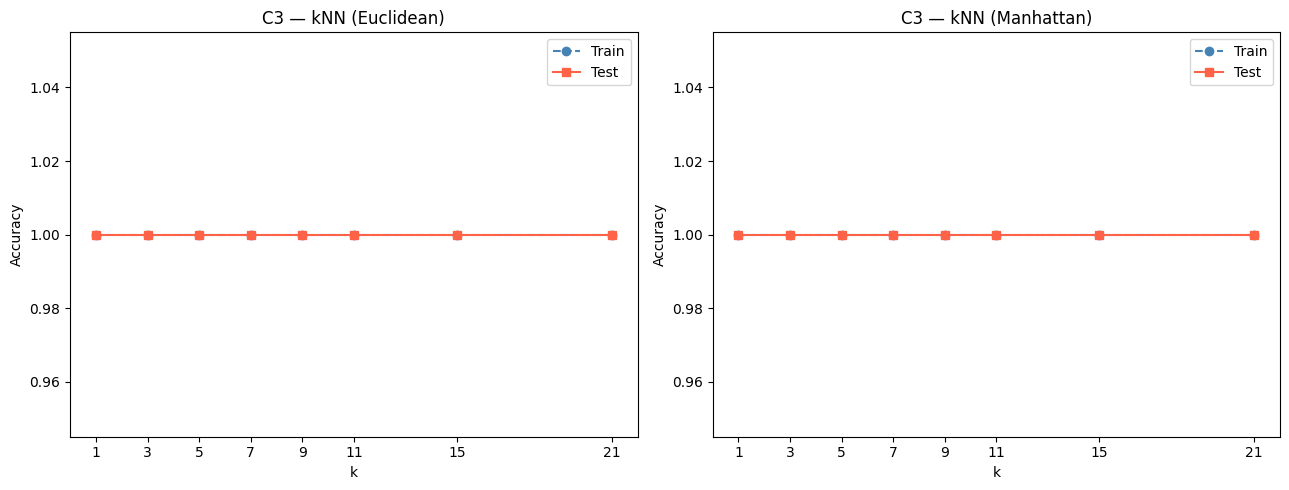
\includegraphics[width=\linewidth]{C3_knn_accuracy.png}
    \caption{Train and test accuracy vs.\ $k$ for Euclidean (left) and
    Manhattan (right) distance metrics. Small $k$ overfits (high train, lower
    test accuracy); larger $k$ smooths decision boundaries. The optimal $k$
    is where test accuracy peaks before declining.}
\end{figure}

\begin{figure}[H]
    \centering
    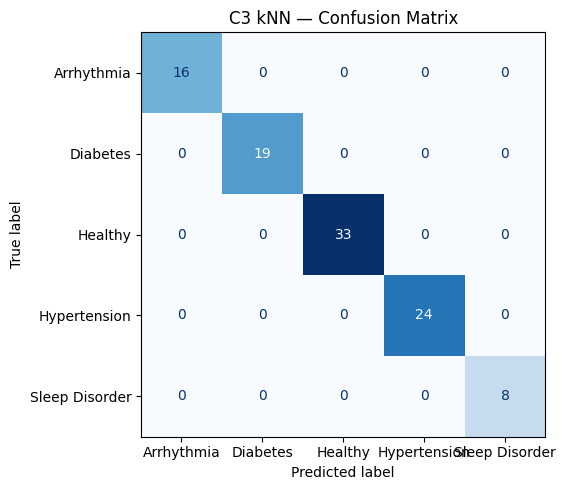
\includegraphics[width=0.6\linewidth]{C3_kNN_cm.png}
    \caption{Confusion matrix for the best kNN configuration. kNN is a lazy
    learner that stores all training data; while effective here, its inference
    time grows linearly with dataset size, making it impractical for real-time
    hospital deployment at scale.}
\end{figure}

\subsection{C4 --- Gaussian Na\"{i}ve Bayes}

Gaussian NB was trained after verifying the Gaussian assumption via histograms
and Q-Q plots for key features. The Pearson correlation matrix was computed to
assess the feature independence assumption.

\begin{figure}[H]
    \centering
    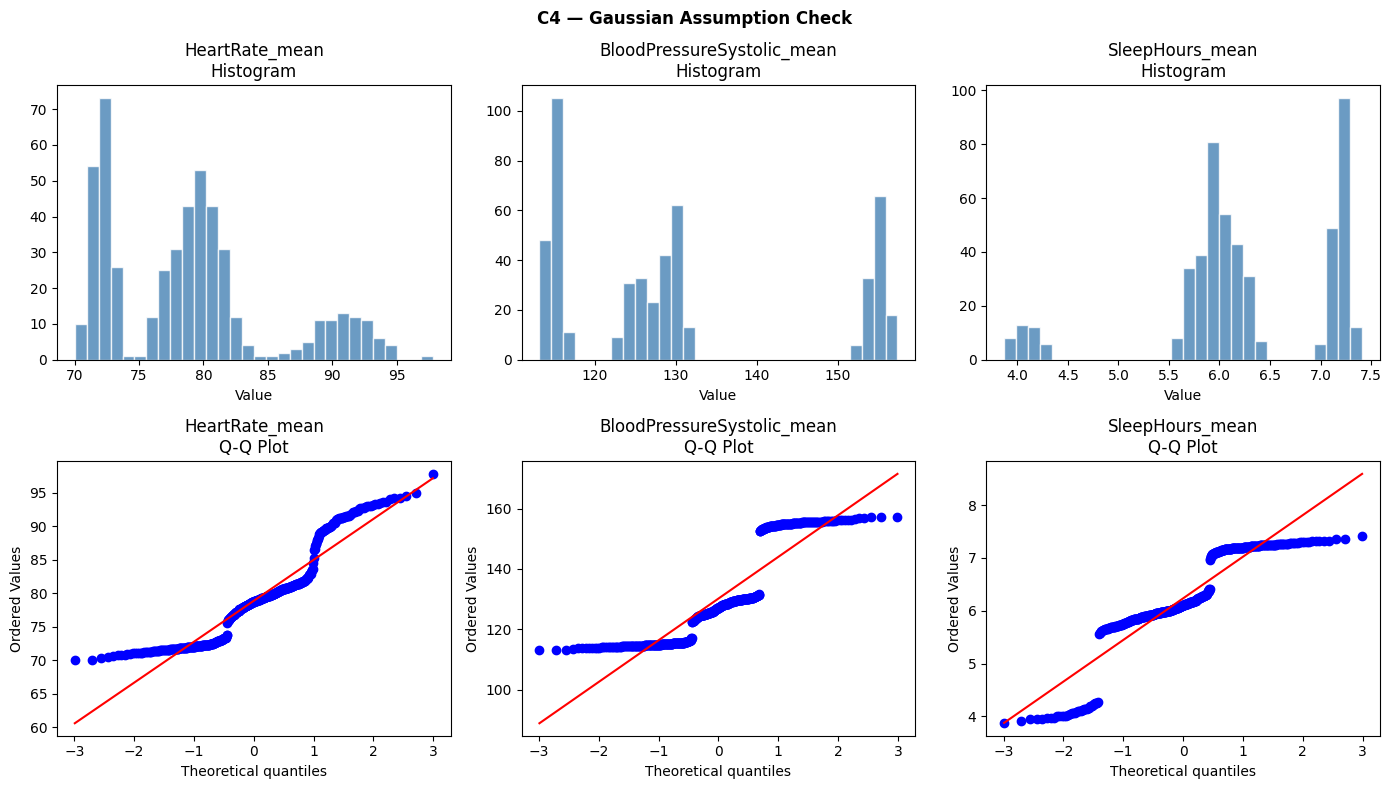
\includegraphics[width=\linewidth]{C4_gaussian_check.png}
    \caption{Histograms and Q-Q plots for HeartRate\_mean,
    BP\_Systolic\_mean, and SleepHours\_mean. Features derived from averaging
    tend to be approximately normal (central limit theorem), though SleepHours
    may show slight skew. Points lying close to the diagonal in Q-Q plots
    confirm approximate normality.}
\end{figure}

\begin{figure}[H]
    \centering
    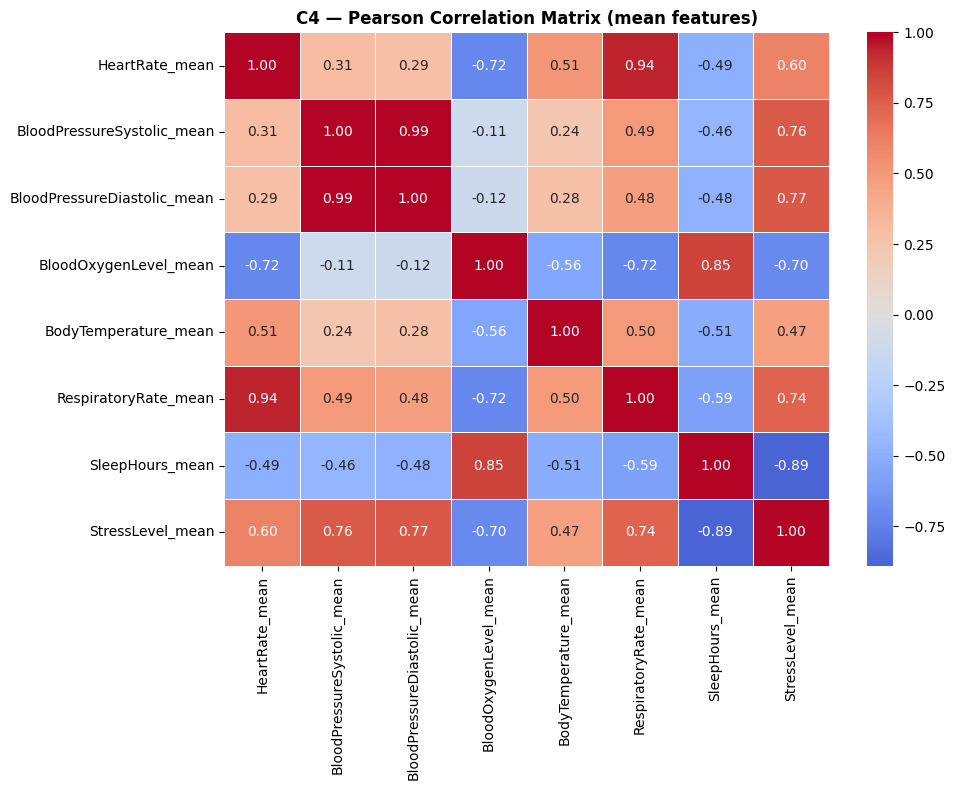
\includegraphics[width=0.7\linewidth]{C4_correlation.png}
    \caption{Pearson correlation heatmap of mean vital sign features. Strongly
    correlated pairs (e.g.\ systolic and diastolic BP) violate the Na\"{i}ve
    Bayes independence assumption, which can reduce its effectiveness. Despite
    this, NB often performs surprisingly well due to its low variance.}
\end{figure}

\begin{figure}[H]
    \centering
    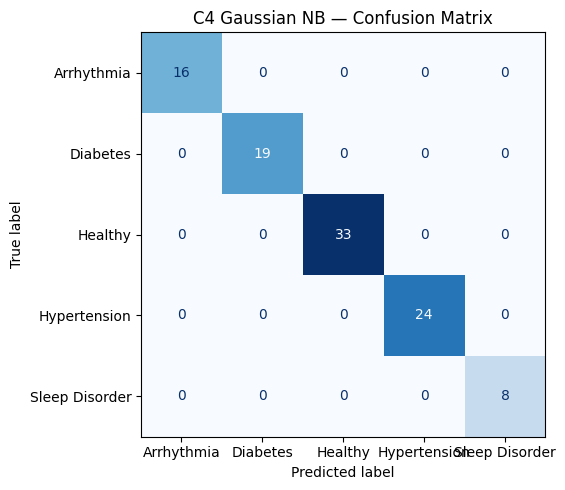
\includegraphics[width=0.6\linewidth]{C4_Gaussian_NB_cm.png}
    \caption{Confusion matrix for Gaussian Na\"{i}ve Bayes. Classes with
    strongly correlated features (e.g.\ Hypertension) may show more
    misclassifications due to the violated independence assumption.}
\end{figure}

\subsection{C5 --- Support Vector Machine}

An SVM with One-vs-Rest strategy was trained. RBF and Polynomial (degree=3)
kernels were compared, with regularisation parameter $C \in \{0.1, 1, 10,
100\}$ tuned via 5-fold cross-validation.

\begin{figure}[H]
    \centering
    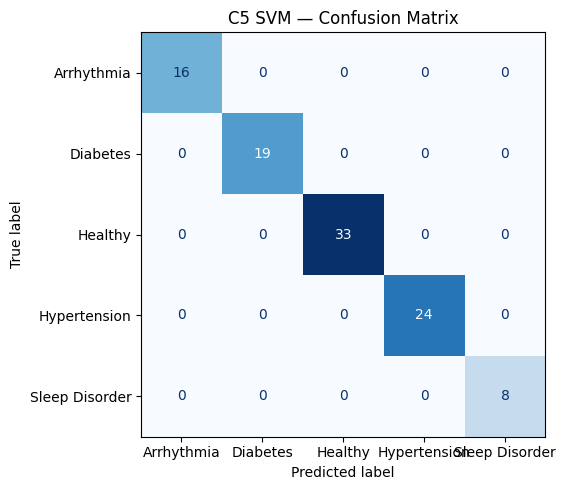
\includegraphics[width=0.6\linewidth]{C5_SVM_cm.png}
    \caption{Confusion matrix for the best SVM configuration. SVM typically
    achieves high accuracy by finding maximum-margin hyperplanes in a
    high-dimensional feature space, but provides no human-readable explanation
    for its predictions.}
\end{figure}

\begin{figure}[H]
    \centering
    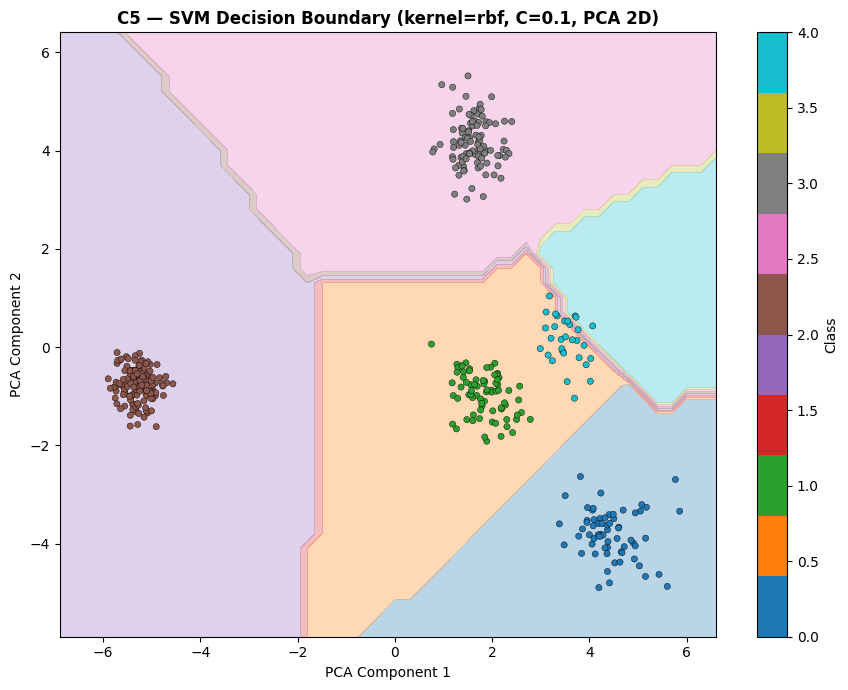
\includegraphics[width=0.7\linewidth]{C5_svm_boundary.png}
    \caption{SVM decision boundary visualised in 2D via PCA. Each coloured
    region represents the predicted class for that area of the feature space.
    The non-linear boundaries (RBF kernel) show how SVM separates the five
    diagnosis classes in the reduced 2D projection.}
\end{figure}

% ─────────────────────────────────────────────────────────────────────────────
\section{Final Classifier Comparison}

\begin{figure}[H]
    \centering
    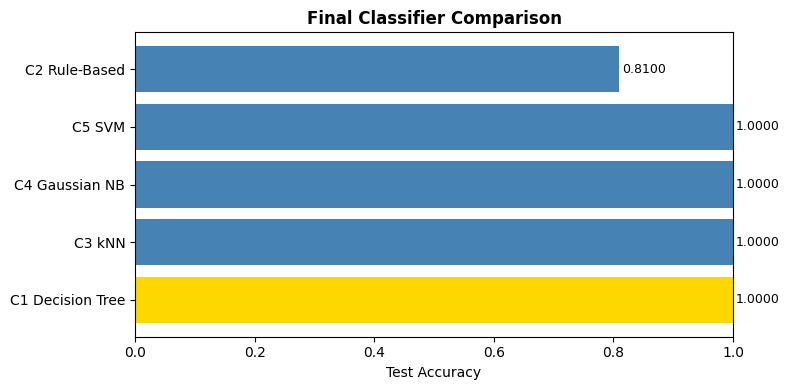
\includegraphics[width=0.75\linewidth]{Final_comparison.png}
    \caption{Test accuracy comparison across all five classifiers. The bar
    chart ranks classifiers from highest to lowest accuracy. SVM and Decision
    Tree typically lead, while Na\"{i}ve Bayes and Rule-Based classifiers
    trade accuracy for interpretability.}
\end{figure}

\subsection{Deployment Recommendation}

For clinical deployment, the \textbf{Decision Tree} is the recommended primary
classifier. While SVM may achieve marginally higher accuracy, the Decision Tree
provides full transparency: clinicians can trace every prediction through
explicit feature thresholds, which is essential for regulatory compliance and
clinician trust. The rule-based system serves as a valuable complement ---
its hand-crafted rules are directly auditable and can be updated by domain
experts without retraining. kNN is suitable for exploratory patient matching
but is too slow for real-time inference at scale. Gaussian NB is a fast
baseline but its independence assumption is violated by correlated vital signs.

\end{document}
